
% Default to the notebook output style

    


% Inherit from the specified cell style.




    
\documentclass[11pt]{article}

    
    
    \usepackage[T1]{fontenc}
    % Nicer default font than Computer Modern for most use cases
    \usepackage{palatino}

    % Basic figure setup, for now with no caption control since it's done
    % automatically by Pandoc (which extracts ![](path) syntax from Markdown).
    \usepackage{graphicx}
    % We will generate all images so they have a width \maxwidth. This means
    % that they will get their normal width if they fit onto the page, but
    % are scaled down if they would overflow the margins.
    \makeatletter
    \def\maxwidth{\ifdim\Gin@nat@width>\linewidth\linewidth
    \else\Gin@nat@width\fi}
    \makeatother
    \let\Oldincludegraphics\includegraphics
    % Set max figure width to be 80% of text width, for now hardcoded.
    \renewcommand{\includegraphics}[1]{\Oldincludegraphics[width=.8\maxwidth]{#1}}
    % Ensure that by default, figures have no caption (until we provide a
    % proper Figure object with a Caption API and a way to capture that
    % in the conversion process - todo).
    \usepackage{caption}
    \DeclareCaptionLabelFormat{nolabel}{}
    \captionsetup{labelformat=nolabel}

    \usepackage{adjustbox} % Used to constrain images to a maximum size 
    \usepackage{xcolor} % Allow colors to be defined
    \usepackage{enumerate} % Needed for markdown enumerations to work
    \usepackage{geometry} % Used to adjust the document margins
    \usepackage{amsmath} % Equations
    \usepackage{amssymb} % Equations
    \usepackage{textcomp} % defines textquotesingle
    % Hack from http://tex.stackexchange.com/a/47451/13684:
    \AtBeginDocument{%
        \def\PYZsq{\textquotesingle}% Upright quotes in Pygmentized code
    }
    \usepackage{upquote} % Upright quotes for verbatim code
    \usepackage{eurosym} % defines \euro
    \usepackage[mathletters]{ucs} % Extended unicode (utf-8) support
    \usepackage[utf8x]{inputenc} % Allow utf-8 characters in the tex document
    \usepackage{fancyvrb} % verbatim replacement that allows latex
    \usepackage{grffile} % extends the file name processing of package graphics 
                         % to support a larger range 
    % The hyperref package gives us a pdf with properly built
    % internal navigation ('pdf bookmarks' for the table of contents,
    % internal cross-reference links, web links for URLs, etc.)
    \usepackage{hyperref}
    \usepackage{longtable} % longtable support required by pandoc >1.10
    \usepackage{booktabs}  % table support for pandoc > 1.12.2
    \usepackage[normalem]{ulem} % ulem is needed to support strikethroughs (\sout)
                                % normalem makes italics be italics, not underlines
    

    
    
    % Colors for the hyperref package
    \definecolor{urlcolor}{rgb}{0,.145,.698}
    \definecolor{linkcolor}{rgb}{.71,0.21,0.01}
    \definecolor{citecolor}{rgb}{.12,.54,.11}

    % ANSI colors
    \definecolor{ansi-black}{HTML}{3E424D}
    \definecolor{ansi-black-intense}{HTML}{282C36}
    \definecolor{ansi-red}{HTML}{E75C58}
    \definecolor{ansi-red-intense}{HTML}{B22B31}
    \definecolor{ansi-green}{HTML}{00A250}
    \definecolor{ansi-green-intense}{HTML}{007427}
    \definecolor{ansi-yellow}{HTML}{DDB62B}
    \definecolor{ansi-yellow-intense}{HTML}{B27D12}
    \definecolor{ansi-blue}{HTML}{208FFB}
    \definecolor{ansi-blue-intense}{HTML}{0065CA}
    \definecolor{ansi-magenta}{HTML}{D160C4}
    \definecolor{ansi-magenta-intense}{HTML}{A03196}
    \definecolor{ansi-cyan}{HTML}{60C6C8}
    \definecolor{ansi-cyan-intense}{HTML}{258F8F}
    \definecolor{ansi-white}{HTML}{C5C1B4}
    \definecolor{ansi-white-intense}{HTML}{A1A6B2}

    % commands and environments needed by pandoc snippets
    % extracted from the output of `pandoc -s`
    \providecommand{\tightlist}{%
      \setlength{\itemsep}{0pt}\setlength{\parskip}{0pt}}
    \DefineVerbatimEnvironment{Highlighting}{Verbatim}{commandchars=\\\{\}}
    % Add ',fontsize=\small' for more characters per line
    \newenvironment{Shaded}{}{}
    \newcommand{\KeywordTok}[1]{\textcolor[rgb]{0.00,0.44,0.13}{\textbf{{#1}}}}
    \newcommand{\DataTypeTok}[1]{\textcolor[rgb]{0.56,0.13,0.00}{{#1}}}
    \newcommand{\DecValTok}[1]{\textcolor[rgb]{0.25,0.63,0.44}{{#1}}}
    \newcommand{\BaseNTok}[1]{\textcolor[rgb]{0.25,0.63,0.44}{{#1}}}
    \newcommand{\FloatTok}[1]{\textcolor[rgb]{0.25,0.63,0.44}{{#1}}}
    \newcommand{\CharTok}[1]{\textcolor[rgb]{0.25,0.44,0.63}{{#1}}}
    \newcommand{\StringTok}[1]{\textcolor[rgb]{0.25,0.44,0.63}{{#1}}}
    \newcommand{\CommentTok}[1]{\textcolor[rgb]{0.38,0.63,0.69}{\textit{{#1}}}}
    \newcommand{\OtherTok}[1]{\textcolor[rgb]{0.00,0.44,0.13}{{#1}}}
    \newcommand{\AlertTok}[1]{\textcolor[rgb]{1.00,0.00,0.00}{\textbf{{#1}}}}
    \newcommand{\FunctionTok}[1]{\textcolor[rgb]{0.02,0.16,0.49}{{#1}}}
    \newcommand{\RegionMarkerTok}[1]{{#1}}
    \newcommand{\ErrorTok}[1]{\textcolor[rgb]{1.00,0.00,0.00}{\textbf{{#1}}}}
    \newcommand{\NormalTok}[1]{{#1}}
    
    % Additional commands for more recent versions of Pandoc
    \newcommand{\ConstantTok}[1]{\textcolor[rgb]{0.53,0.00,0.00}{{#1}}}
    \newcommand{\SpecialCharTok}[1]{\textcolor[rgb]{0.25,0.44,0.63}{{#1}}}
    \newcommand{\VerbatimStringTok}[1]{\textcolor[rgb]{0.25,0.44,0.63}{{#1}}}
    \newcommand{\SpecialStringTok}[1]{\textcolor[rgb]{0.73,0.40,0.53}{{#1}}}
    \newcommand{\ImportTok}[1]{{#1}}
    \newcommand{\DocumentationTok}[1]{\textcolor[rgb]{0.73,0.13,0.13}{\textit{{#1}}}}
    \newcommand{\AnnotationTok}[1]{\textcolor[rgb]{0.38,0.63,0.69}{\textbf{\textit{{#1}}}}}
    \newcommand{\CommentVarTok}[1]{\textcolor[rgb]{0.38,0.63,0.69}{\textbf{\textit{{#1}}}}}
    \newcommand{\VariableTok}[1]{\textcolor[rgb]{0.10,0.09,0.49}{{#1}}}
    \newcommand{\ControlFlowTok}[1]{\textcolor[rgb]{0.00,0.44,0.13}{\textbf{{#1}}}}
    \newcommand{\OperatorTok}[1]{\textcolor[rgb]{0.40,0.40,0.40}{{#1}}}
    \newcommand{\BuiltInTok}[1]{{#1}}
    \newcommand{\ExtensionTok}[1]{{#1}}
    \newcommand{\PreprocessorTok}[1]{\textcolor[rgb]{0.74,0.48,0.00}{{#1}}}
    \newcommand{\AttributeTok}[1]{\textcolor[rgb]{0.49,0.56,0.16}{{#1}}}
    \newcommand{\InformationTok}[1]{\textcolor[rgb]{0.38,0.63,0.69}{\textbf{\textit{{#1}}}}}
    \newcommand{\WarningTok}[1]{\textcolor[rgb]{0.38,0.63,0.69}{\textbf{\textit{{#1}}}}}
    
    
    % Define a nice break command that doesn't care if a line doesn't already
    % exist.
    \def\br{\hspace*{\fill} \\* }
    % Math Jax compatability definitions
    \def\gt{>}
    \def\lt{<}
    % Document parameters
    \title{p}
    
    
    

    % Pygments definitions
    
\makeatletter
\def\PY@reset{\let\PY@it=\relax \let\PY@bf=\relax%
    \let\PY@ul=\relax \let\PY@tc=\relax%
    \let\PY@bc=\relax \let\PY@ff=\relax}
\def\PY@tok#1{\csname PY@tok@#1\endcsname}
\def\PY@toks#1+{\ifx\relax#1\empty\else%
    \PY@tok{#1}\expandafter\PY@toks\fi}
\def\PY@do#1{\PY@bc{\PY@tc{\PY@ul{%
    \PY@it{\PY@bf{\PY@ff{#1}}}}}}}
\def\PY#1#2{\PY@reset\PY@toks#1+\relax+\PY@do{#2}}

\expandafter\def\csname PY@tok@gd\endcsname{\def\PY@tc##1{\textcolor[rgb]{0.63,0.00,0.00}{##1}}}
\expandafter\def\csname PY@tok@gu\endcsname{\let\PY@bf=\textbf\def\PY@tc##1{\textcolor[rgb]{0.50,0.00,0.50}{##1}}}
\expandafter\def\csname PY@tok@gt\endcsname{\def\PY@tc##1{\textcolor[rgb]{0.00,0.27,0.87}{##1}}}
\expandafter\def\csname PY@tok@gs\endcsname{\let\PY@bf=\textbf}
\expandafter\def\csname PY@tok@gr\endcsname{\def\PY@tc##1{\textcolor[rgb]{1.00,0.00,0.00}{##1}}}
\expandafter\def\csname PY@tok@cm\endcsname{\let\PY@it=\textit\def\PY@tc##1{\textcolor[rgb]{0.25,0.50,0.50}{##1}}}
\expandafter\def\csname PY@tok@vg\endcsname{\def\PY@tc##1{\textcolor[rgb]{0.10,0.09,0.49}{##1}}}
\expandafter\def\csname PY@tok@vi\endcsname{\def\PY@tc##1{\textcolor[rgb]{0.10,0.09,0.49}{##1}}}
\expandafter\def\csname PY@tok@mh\endcsname{\def\PY@tc##1{\textcolor[rgb]{0.40,0.40,0.40}{##1}}}
\expandafter\def\csname PY@tok@cs\endcsname{\let\PY@it=\textit\def\PY@tc##1{\textcolor[rgb]{0.25,0.50,0.50}{##1}}}
\expandafter\def\csname PY@tok@ge\endcsname{\let\PY@it=\textit}
\expandafter\def\csname PY@tok@vc\endcsname{\def\PY@tc##1{\textcolor[rgb]{0.10,0.09,0.49}{##1}}}
\expandafter\def\csname PY@tok@il\endcsname{\def\PY@tc##1{\textcolor[rgb]{0.40,0.40,0.40}{##1}}}
\expandafter\def\csname PY@tok@go\endcsname{\def\PY@tc##1{\textcolor[rgb]{0.53,0.53,0.53}{##1}}}
\expandafter\def\csname PY@tok@cp\endcsname{\def\PY@tc##1{\textcolor[rgb]{0.74,0.48,0.00}{##1}}}
\expandafter\def\csname PY@tok@gi\endcsname{\def\PY@tc##1{\textcolor[rgb]{0.00,0.63,0.00}{##1}}}
\expandafter\def\csname PY@tok@gh\endcsname{\let\PY@bf=\textbf\def\PY@tc##1{\textcolor[rgb]{0.00,0.00,0.50}{##1}}}
\expandafter\def\csname PY@tok@ni\endcsname{\let\PY@bf=\textbf\def\PY@tc##1{\textcolor[rgb]{0.60,0.60,0.60}{##1}}}
\expandafter\def\csname PY@tok@nl\endcsname{\def\PY@tc##1{\textcolor[rgb]{0.63,0.63,0.00}{##1}}}
\expandafter\def\csname PY@tok@nn\endcsname{\let\PY@bf=\textbf\def\PY@tc##1{\textcolor[rgb]{0.00,0.00,1.00}{##1}}}
\expandafter\def\csname PY@tok@no\endcsname{\def\PY@tc##1{\textcolor[rgb]{0.53,0.00,0.00}{##1}}}
\expandafter\def\csname PY@tok@na\endcsname{\def\PY@tc##1{\textcolor[rgb]{0.49,0.56,0.16}{##1}}}
\expandafter\def\csname PY@tok@nb\endcsname{\def\PY@tc##1{\textcolor[rgb]{0.00,0.50,0.00}{##1}}}
\expandafter\def\csname PY@tok@nc\endcsname{\let\PY@bf=\textbf\def\PY@tc##1{\textcolor[rgb]{0.00,0.00,1.00}{##1}}}
\expandafter\def\csname PY@tok@nd\endcsname{\def\PY@tc##1{\textcolor[rgb]{0.67,0.13,1.00}{##1}}}
\expandafter\def\csname PY@tok@ne\endcsname{\let\PY@bf=\textbf\def\PY@tc##1{\textcolor[rgb]{0.82,0.25,0.23}{##1}}}
\expandafter\def\csname PY@tok@nf\endcsname{\def\PY@tc##1{\textcolor[rgb]{0.00,0.00,1.00}{##1}}}
\expandafter\def\csname PY@tok@si\endcsname{\let\PY@bf=\textbf\def\PY@tc##1{\textcolor[rgb]{0.73,0.40,0.53}{##1}}}
\expandafter\def\csname PY@tok@s2\endcsname{\def\PY@tc##1{\textcolor[rgb]{0.73,0.13,0.13}{##1}}}
\expandafter\def\csname PY@tok@nt\endcsname{\let\PY@bf=\textbf\def\PY@tc##1{\textcolor[rgb]{0.00,0.50,0.00}{##1}}}
\expandafter\def\csname PY@tok@nv\endcsname{\def\PY@tc##1{\textcolor[rgb]{0.10,0.09,0.49}{##1}}}
\expandafter\def\csname PY@tok@s1\endcsname{\def\PY@tc##1{\textcolor[rgb]{0.73,0.13,0.13}{##1}}}
\expandafter\def\csname PY@tok@ch\endcsname{\let\PY@it=\textit\def\PY@tc##1{\textcolor[rgb]{0.25,0.50,0.50}{##1}}}
\expandafter\def\csname PY@tok@m\endcsname{\def\PY@tc##1{\textcolor[rgb]{0.40,0.40,0.40}{##1}}}
\expandafter\def\csname PY@tok@gp\endcsname{\let\PY@bf=\textbf\def\PY@tc##1{\textcolor[rgb]{0.00,0.00,0.50}{##1}}}
\expandafter\def\csname PY@tok@sh\endcsname{\def\PY@tc##1{\textcolor[rgb]{0.73,0.13,0.13}{##1}}}
\expandafter\def\csname PY@tok@ow\endcsname{\let\PY@bf=\textbf\def\PY@tc##1{\textcolor[rgb]{0.67,0.13,1.00}{##1}}}
\expandafter\def\csname PY@tok@sx\endcsname{\def\PY@tc##1{\textcolor[rgb]{0.00,0.50,0.00}{##1}}}
\expandafter\def\csname PY@tok@bp\endcsname{\def\PY@tc##1{\textcolor[rgb]{0.00,0.50,0.00}{##1}}}
\expandafter\def\csname PY@tok@c1\endcsname{\let\PY@it=\textit\def\PY@tc##1{\textcolor[rgb]{0.25,0.50,0.50}{##1}}}
\expandafter\def\csname PY@tok@o\endcsname{\def\PY@tc##1{\textcolor[rgb]{0.40,0.40,0.40}{##1}}}
\expandafter\def\csname PY@tok@kc\endcsname{\let\PY@bf=\textbf\def\PY@tc##1{\textcolor[rgb]{0.00,0.50,0.00}{##1}}}
\expandafter\def\csname PY@tok@c\endcsname{\let\PY@it=\textit\def\PY@tc##1{\textcolor[rgb]{0.25,0.50,0.50}{##1}}}
\expandafter\def\csname PY@tok@mf\endcsname{\def\PY@tc##1{\textcolor[rgb]{0.40,0.40,0.40}{##1}}}
\expandafter\def\csname PY@tok@err\endcsname{\def\PY@bc##1{\setlength{\fboxsep}{0pt}\fcolorbox[rgb]{1.00,0.00,0.00}{1,1,1}{\strut ##1}}}
\expandafter\def\csname PY@tok@mb\endcsname{\def\PY@tc##1{\textcolor[rgb]{0.40,0.40,0.40}{##1}}}
\expandafter\def\csname PY@tok@ss\endcsname{\def\PY@tc##1{\textcolor[rgb]{0.10,0.09,0.49}{##1}}}
\expandafter\def\csname PY@tok@sr\endcsname{\def\PY@tc##1{\textcolor[rgb]{0.73,0.40,0.53}{##1}}}
\expandafter\def\csname PY@tok@mo\endcsname{\def\PY@tc##1{\textcolor[rgb]{0.40,0.40,0.40}{##1}}}
\expandafter\def\csname PY@tok@kd\endcsname{\let\PY@bf=\textbf\def\PY@tc##1{\textcolor[rgb]{0.00,0.50,0.00}{##1}}}
\expandafter\def\csname PY@tok@mi\endcsname{\def\PY@tc##1{\textcolor[rgb]{0.40,0.40,0.40}{##1}}}
\expandafter\def\csname PY@tok@kn\endcsname{\let\PY@bf=\textbf\def\PY@tc##1{\textcolor[rgb]{0.00,0.50,0.00}{##1}}}
\expandafter\def\csname PY@tok@cpf\endcsname{\let\PY@it=\textit\def\PY@tc##1{\textcolor[rgb]{0.25,0.50,0.50}{##1}}}
\expandafter\def\csname PY@tok@kr\endcsname{\let\PY@bf=\textbf\def\PY@tc##1{\textcolor[rgb]{0.00,0.50,0.00}{##1}}}
\expandafter\def\csname PY@tok@s\endcsname{\def\PY@tc##1{\textcolor[rgb]{0.73,0.13,0.13}{##1}}}
\expandafter\def\csname PY@tok@kp\endcsname{\def\PY@tc##1{\textcolor[rgb]{0.00,0.50,0.00}{##1}}}
\expandafter\def\csname PY@tok@w\endcsname{\def\PY@tc##1{\textcolor[rgb]{0.73,0.73,0.73}{##1}}}
\expandafter\def\csname PY@tok@kt\endcsname{\def\PY@tc##1{\textcolor[rgb]{0.69,0.00,0.25}{##1}}}
\expandafter\def\csname PY@tok@sc\endcsname{\def\PY@tc##1{\textcolor[rgb]{0.73,0.13,0.13}{##1}}}
\expandafter\def\csname PY@tok@sb\endcsname{\def\PY@tc##1{\textcolor[rgb]{0.73,0.13,0.13}{##1}}}
\expandafter\def\csname PY@tok@k\endcsname{\let\PY@bf=\textbf\def\PY@tc##1{\textcolor[rgb]{0.00,0.50,0.00}{##1}}}
\expandafter\def\csname PY@tok@se\endcsname{\let\PY@bf=\textbf\def\PY@tc##1{\textcolor[rgb]{0.73,0.40,0.13}{##1}}}
\expandafter\def\csname PY@tok@sd\endcsname{\let\PY@it=\textit\def\PY@tc##1{\textcolor[rgb]{0.73,0.13,0.13}{##1}}}

\def\PYZbs{\char`\\}
\def\PYZus{\char`\_}
\def\PYZob{\char`\{}
\def\PYZcb{\char`\}}
\def\PYZca{\char`\^}
\def\PYZam{\char`\&}
\def\PYZlt{\char`\<}
\def\PYZgt{\char`\>}
\def\PYZsh{\char`\#}
\def\PYZpc{\char`\%}
\def\PYZdl{\char`\$}
\def\PYZhy{\char`\-}
\def\PYZsq{\char`\'}
\def\PYZdq{\char`\"}
\def\PYZti{\char`\~}
% for compatibility with earlier versions
\def\PYZat{@}
\def\PYZlb{[}
\def\PYZrb{]}
\makeatother


    % Exact colors from NB
    \definecolor{incolor}{rgb}{0.0, 0.0, 0.5}
    \definecolor{outcolor}{rgb}{0.545, 0.0, 0.0}
    
    \usepackage[framemethod=tikz]{mdframed}



    
    % Prevent overflowing lines due to hard-to-break entities
    \sloppy 
    % Setup hyperref package
    \hypersetup{
      breaklinks=true,  % so long urls are correctly broken across lines
      colorlinks=true,
      urlcolor=urlcolor,
      linkcolor=linkcolor,
      citecolor=citecolor,
      }
    % Slightly bigger margins than the latex defaults
    
    \geometry{verbose,tmargin=1in,bmargin=1in,lmargin=1in,rmargin=1in}
    
    

    \begin{document}
    
    
    \maketitle
    
    

    
    \section{Table of Contents}\label{table-of-contents}

{1~~}Resumen teórico

{1.1~~}Nociones sobre la distribución t de Student

{1.2~~}Nociones sobre test de hipótesis sobre 1 población

{1.2.1~~}Concepto de p-valor

{1.2.2~~}Tipos de tests de hipótesis

{1.2.3~~}Cómo se cálcula el p-valor

{1.2.4~~}Pasos para el diseño de un test de hipótesis

{1.3~~}Nociones sobre test de hipótesis sobre 2 poblaciones

{1.3.1~~}t-test pareado

{1.4~~}Nociones sobre comparación y replicación de clasificadores

{1.4.1~~}Introducción

{1.4.2~~}Métodos de muestreo

{1.4.3~~}Test de hipótesis más comunmente aplicados en este problema

{2~~}Ejecución práctica

{2.1~~}Descripción del experimento

{2.2~~}Diseño del test en el contexto del problema

{2.3~~}Realización del experimento

{2.3.1~~}Generación de particiones y bloques

{2.3.2~~}Evaluación de los clasificadores en cada bloque de cada
partición

{2.3.3~~}Resultados de las evaluaciones ordenados por bloque - con
medias y desviación típica

{2.3.4~~}Tabla de diferencias tras la ordenación

{2.3.5~~}Prueba de la normalidad de las diferencias

{2.3.6~~}Realización del t-test

{3~~}Conclusiones

{4~~}Referencias

    \section{Resumen teórico}\label{resumen-teuxf3rico}

\subsection{Nociones sobre la distribución t de
Student}\label{nociones-sobre-la-distribuciuxf3n-t-de-student}

\textbf{La distribución t de Student} es una distribución de
probabilidad que \textbf{se utiliza para estimar los parámetros de una
población cuando el tamaño de la muestra es pequeño y/o cuando la
varianza de la población es desconocida}.

En estadística, \textbf{un estadístico (muestral) es una función
medible} \(T\) que, dada una muestra estadística de valores
\((X_1,X_2,...,X_n)\), les asigna un número, \(T(X_1,X_2,...,X_n)\),
\textbf{que sirve para estimar determinado parámetro de la distribución
de la que procede la muestra}.

Cuando se extrae una muestra de tamaño \(n\) de una población que tiene
una distribución normal (o casi normal), la media de la muestra puede
transformarse en un estadístico \(t\), utilizando la ecuación:

\[ t = \frac{ \overline{x} - \mu}{s / \sqrt{n}}  \]

dónde

\begin{itemize}
\tightlist
\item
  \(\overline{x}\) es la media de la muestra
\item
  \(\mu\) es la media de la población
\item
  \(s\) es la desviación estándar de la muestra
\item
  \(n\) es el tamaño de la muestra
\item
  \(n - 1\) son los grados de libertad
\end{itemize}

El estadístico \(t\) producido por esta transformación puede asociarse
con una función de probabilidad única.

\textbf{Esta probabilidad acumulativa representa la probabilidad de
encontrar una media de muestra menor o igual que \(x\), dada una muestra
aleatoria de tamaño \(n\).}

En realidad hay muchas distribuciones t de Student. La forma particular
de la distribución t está determinada por sus \textbf{grados de
libertad}, que se suelen denotar por \(v\). Los grados de libertad se
refieren al número de observaciones independientes en un conjunto de
datos. El número de observaciones independientes es igual al tamaño de
la muestra menos uno. Por lo tanto, la distribución t de Student de las
muestras de tamaño 8 se describiría por una distribución t con 8 - 1 o 7
grados de libertad. De forma similar, se utilizaría una distribución t
con 15 grados de libertad con una muestra de tamaño 16.

\begin{figure}
\centering
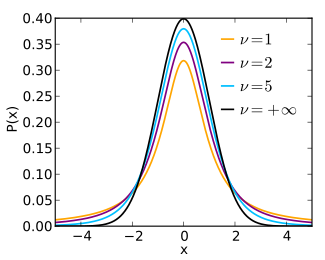
\includegraphics{student_t_pdf.png}
\caption{Distribución t de Student}
\end{figure}

\emph{Figura: distribución de probabilidad t de Student para varios
grados de libertad}

La distribución de probabilidad t de Student \textbf{tiene las
siguientes propiedades}:

\begin{itemize}
\tightlist
\item
  La media de la distribución es igual a 0
\item
  La varianza es igual a v / (v - 2), donde v es el grado de libertad de
  la distribución y v\textgreater{} 2.
\item
  La varianza es siempre mayor que 1, aunque está cerca de 1 cuando hay
  muchos grados de libertad. Con infinitos grados de libertad, la
  distribución t es la misma que la distribución normal estándar.
\end{itemize}

La distribución \textbf{t de Student puede usarse si se da alguna de las
siguientes condiciones}:

\begin{itemize}
\tightlist
\item
  La distribución de la población es normal
\item
  La distribución de la población es simétrica, unimodal, sin valores
  atípicos, y el tamaño de la muestra es de al menos 30
\item
  La distribución de la población es moderadamente sesgada, unimodal,
  sin valores atípicos, y el tamaño de la muestra es de al menos 40
\item
  El tamaño de la muestra es mayor que 40, sin valores atípicos
\end{itemize}

La distribución t no se debe utilizar con muestras pequeñas de
poblaciones que no son aproximadamente normales.

La distribución de probabilidad t de Student \textbf{tiene las
siguientes aplicaciones}:

\begin{itemize}
\tightlist
\item
  Test de Hipótesis de la media poblacional
\item
  Test de Hipótesis de la diferencia entre las medias de dos poblaciones
\item
  Test de Hipótesis de la diferencia entre las medias de dos poblaciones
  con muestras dependientes (paired t-test)
\item
  Test de Hipótesis sobre el coeficiente de correlación
\end{itemize}

    \subsection{Nociones sobre test de hipótesis sobre 1
población}\label{nociones-sobre-test-de-hipuxf3tesis-sobre-1-poblaciuxf3n}

Lost Tests de Hipótesis son una prueba estadística utilizada para
determinar si una hipótesis asumida para una muestra de datos es
verdadera para toda la población o no.

Lost Tests de Hipótesis formulan dos hipótesis opuestas sobre una
población: \textbf{la hipótesis nula \(H_0\) y la hipótesis alternativa
\(H_1\)}. La hipótesis nula es la afirmación de que no hay diferencia
entre el estadístico de muestra y el parámetro de la población real y es
la que se prueba. Mientras, la hipótesis alternativa es la afirmación
que es verdadera si se rechaza la hipótesis nula.

\textbf{Basándose en los datos de la muestra, el Test de Hipótesis
determina si se rechaza o no la hipótesis nula.}

Cuando se diseña un test de hipótesis hay que asumir dos tipo de
errores, sobre los que podemos definir dos tipos de parámetros:

\begin{itemize}
\tightlist
\item
  \textbf{Error de tipo I:} la hipótesis nula es rechazada cuando
  debería ser aceptada. El parámetro \(\alpha\) determina la
  probabilididad de que se presente este error que estamos dispuestos a
  asumir en nuestro test
\item
  \textbf{Error de tipo II:} la hipótesis nula es aceptada cuando
  debería ser rechazada. El parámetro \(\beta\) determina la
  probabilididad de que se presente este error que estamos dispuestos a
  asumir en nuestro test
\end{itemize}

Podemos ver los conceptos anteriores gráficamente:

\begin{figure}
\centering
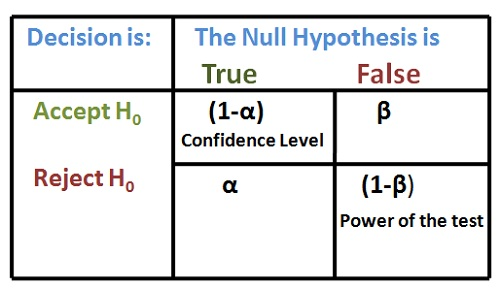
\includegraphics{Hypothesis_Testing.jpg}
\caption{Tipos de error}
\end{figure}

\emph{Figura: tipos de error en los test de hipótesis y parámetros
asociados}

Se definen igualmente:

\begin{itemize}
\tightlist
\item
  el \textbf{Nivel de Confianza del test} \((1-\alpha)\), que representa
  la probabilidad de aceptar la hipótesis nula cuando es verdadera.
\item
  la \textbf{Potencia del test} \((1-\beta)\), que representa la
  probabilidad de rechazar la hipótesis nula cuando es falsa.
\end{itemize}

\subsubsection{Concepto de p-valor}\label{concepto-de-p-valor}

Definimos el \textbf{p-valor como la probabilidad de que, suponiendo
cierta H0, el estadístico de contraste tome un valor al menos tan
extremo como el que se obtiene a partir de las observaciones
muestrales}, i.e., el p-valor es el área de la cola de la distribución
(o colas si el test es bilateral) definida a partir del estadístico de
contraste:. Notas:

\begin{enumerate}
\def\labelenumi{\arabic{enumi}.}
\tightlist
\item
  El p-valor sólo puede calcularse una vez tomada la muestra,
  obteniéndose niveles críticos distintos para cada muestra.
\item
  El p-valor puede interpretarse como un nivel mínimo de significación
  en el sentido de que niveles de significación α , iguales o superiores
  al p - valor llevarán a rechazar la hipótesis nula. Por tanto, cuanto
  menor sea el p - valor mayor es el grado de incompatibilidad de la
  muestra con H0, lo que lleva a rechazar H0.
\item
  El cálculo del p-valor no proporciona de modo sistemático una decisión
  entre H0 y H1. Esta forma de abordar los tests, nos permite una visión
  más amplia, por cuanto nos da información de para qué niveles de
  significación puede rechazarse la hipótesis nula, y para cuales no se
  puede.
\end{enumerate}

\textbf{El p-valor nos proporciona el grado de credibilidad de la
hipótesis nula:}

\begin{itemize}
\tightlist
\item
  si el valor de p fuese ``muy pequeño'' (inferior a 0,001),
  significaría que la hipótesis nula es del todo increíble (en base a
  las observaciones obtenidas), y por tanto la descartaríamos
\item
  si el valor de p oscilase entre 0,05 y 0,001 significaría que hay
  fuertes evidencias en contra de la hipótesis nula, por lo que la
  rechazaríamos o no en función del valor que hubiésemos asignado (a
  priori) a α
\item
  si el valor de p es ``grande'' (superior a 0,05), no habría motivos
  suficientes como para descartar la hipótesis nula, por lo que la
  tomaríamos como cierta.
\end{itemize}

\subsubsection{Tipos de tests de
hipótesis}\label{tipos-de-tests-de-hipuxf3tesis}

Los hay de una cola o unilaterales (por la izquierda o por la derecha) y
de dos colas o bilaterales.

\begin{itemize}
\tightlist
\item
  \textbf{test de una cola por la derecha:} compara la hipótesis de un
  valor mayor en el parámetro que el de la hipótesis nula. El nivel de
  significancia se carga todo hacia el lado derecho, para definir las
  regiones de aceptación y de rechazo.
\item
  \textbf{test de una cola por la izquierda:} compara la hipótesis de un
  valor menor en el parámetro que el de la hipótesis nula. El nivel de
  significancia se carga todo hacia el lado izquierdo, para definir las
  regiones de aceptación y de rechazo.
\item
  \textbf{test bilateral:} compara la hipótesis de un valor igual en el
  parámetro que el de la hipótesis nula. El nivel de significancia se
  carga hacia ambos lados, para definir las regiones de aceptación y de
  rechazo.
\end{itemize}

\[ \] 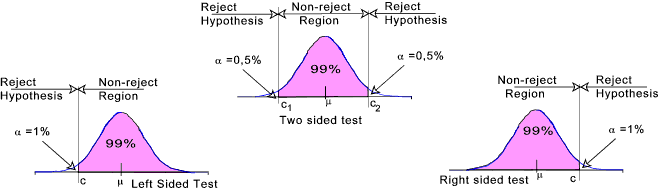
\includegraphics{stat_83.png} \[ \]

\emph{Figura: distintos tipos de test de hipótesis}

\subsubsection{Cómo se cálcula el
p-valor}\label{cuxf3mo-se-cuxe1lcula-el-p-valor}

Depende del tipo de contraste (bilateral, unilateral cola izquierda,
unilateral cola derecha) y del estadístico del contraste. En cualquier
caso, asumimos que vamos a trabajar con la distribución t de Student tal
como se indica en el enunciado de la práctica.

Para una cola unilateral por la derecha,
\(H_0: estadístico \le x; H_1: estadístico \gt x\),
\(p = P(t_{n-1} \gt t_0)\)

Para una cola unilateral por la izquierda,
\(H_0: estadístico \ge x; H_1: estadístico \lt x\),
\(p = P(t_{n-1} \lt t_0)\)

Para una cola bilateral,
\(H_0: estadístico = x; H_1: estadístico \ne x\),
\(p = 2 * P(t_{n-1} \gt \vert t_0 \vert)\)

\subsubsection{Pasos para el diseño de un test de
hipótesis}\label{pasos-para-el-diseuxf1o-de-un-test-de-hipuxf3tesis}

Son los siguientes:

\begin{enumerate}
\def\labelenumi{\arabic{enumi}.}
\tightlist
\item
  Identificar el parámetro de interés (\(\mu\) → media poblacional)
\item
  Establecer las hipótesis \(H_0\) y \(H_1\).
\item
  Fijar un nivel de significación \(\alpha\)
\item
  Determinar el estadístico del contraste
\item
  Establecer las regiones de aceptación y rechazo
\item
  Calcular el valor que toma el estadístico del contraste para la
  muestra seleccionada.
\item
  Decidir si debe o no rechazarse \(H_0\) e interpretar la decisión
  tomada
\end{enumerate}

    \subsection{Nociones sobre test de hipótesis sobre 2
poblaciones}\label{nociones-sobre-test-de-hipuxf3tesis-sobre-2-poblaciones}

Un test de hipótesis para dos muestras es similar en muchos aspectos al
test para una muestra:

\begin{itemize}
\tightlist
\item
  Se especifica una hipótesis nula, en la mayoría de los casos se
  propone que las medias de las dos poblaciones son iguales y se
  establece la hipótesis alternativa (uni o bilateral)
\item
  Se especifica un nivel de significación \(\alpha\)
\item
  Se calcula el p-valor: la probabilidad de obtener datos cuyas medias
  muestrales difieren tanto o más que la diferencia observada cuando
  \(H_0\) es verdadera. Si esta probabilidad es pequeña (menor que
  \(\alpha\)) se rechaza \(H_0\) y se concluye que la diferencia
  observada no es atribuible al azar y las medias de las dos poblaciones
  son diferentes.
\end{itemize}

\textbf{El estadístico del test dependerá de la estructura de los
conjuntos de datos. En particular es importante establecer si los datos
corresponden a muestras apareadas o independientes.}

Dos muestras son independientes o dependientes entre sí, en función de
si las observaciones de las muestras se han obtenido de los mismos
individuos u objetos o no.

Si ambas muestras se obtienen de distintos individuos, máquinas,
empresas, objetos, etc., no hay nada en común en dichas muestras lo que
hace que ambas sean \textbf{``independientes''}.

Sin embargo, si las observaciones o valores de ambas muestras se
obtienen de los mismos individuos, empresas, agentes, etc.
(potencialmente sujetos a algún tipo de acción entre muestra y muestra),
diremos que hay algo en común en dichas muestras por lo que serán
muestras \textbf{``dependientes'' o ``no independientes''}.

\subsubsection{t-test pareado}\label{t-test-pareado}

Si se quiere comparar estadísticos sobre dos poblaciones distintas, una
forma de hacerlo es hacer un t-test de una población sobre la muestra
resultante de practicar las diferencias a las dos muestras de las 2
poblaciones originales. Esto es lo que se conoce como paired t-test.

Atendiendo a la enciclopedia matemática on-line
\href{http://mathworld.wolfram.com/Pairedt-Test.html}{Mathworld}, dados
dos conjuntos \(X_i\) e \(Y_i\) de n muestras cada uno, el
\textbf{t-test pareado} determina si se diferencian unas de otras de una
manera significativa bajo las suposiciones de que las diferencias de los
pares son independientes y normalmente distribuidas.

Para aplicar la prueba, se define:

\begin{itemize}
\tightlist
\item
  \(\hat{X}_{i} = (X_{i} - \overline{X})\)
\item
  \(\hat{Y}_{i} = (Y_{i} - \overline{Y})\)
\end{itemize}

de dónde se construye el estadístico:

\[t = (\overline{X} - \overline{Y}) \sqrt{\frac{n (n-1)}{\sum_{i=1}^n (\hat{X}_{i} - \hat{Y}_{i})^2}}\]

Este estadístico tiene una distribución t-Student con n-1 grados de
libertad.

    \subsection{Nociones sobre comparación y replicación de
clasificadores}\label{nociones-sobre-comparaciuxf3n-y-replicaciuxf3n-de-clasificadores}

Resumimos aquí las partes más relevantes del artículo \textbf{Bouckaert,
R. (2004). Estimating Replicability of Classifier Learning Experiments,
ICML,} en relación con los ejercicios pedidos en esta práctica.

\subsubsection{Introducción}\label{introducciuxf3n}

\begin{quote}
\textbf{Definición}: la \textbf{replicabilidad de un experimento} es la
probabilidad de dos ejecuciones del experimento en el mismo conjunto de
datos, con el mismo par de algoritmos y el mismo método de muestreo de
los datos produzca el mismo resultado.
\end{quote}

El problema que se aborda es, dados dos algoritmos de aprendizaje \(A\)
y \(B\) que generan clasificadores y un pequeño conjunto de datos \(D\),
cómo tomar una decisión sobre cuál de los dos algoritmos funciona mejor
basado en la precisión de clasificación para el conjunto de datos dado.
Un método general para tomar tal decisión es dividir \(D\) en un
conjunto de entrenamiento \(D_t\) y un conjunto de prueba \(D - D_t\).
Luego, se entrena el algoritmo \(A\) y \(B\) en \(D_t\) y se registra la
exactitud de clasificación en el \(D - D_t\). De esta manera, obtenemos
dos precisiones de clasificación \(P_A\) y \(P_B\) y la diferencia
\(x = P_A - P_B\) nos da una indicación de qué algoritmo ofrece mejor
rendimiento.

Una manera formal de tomar tal decisión es aplicar un test de hipótesis.
Sin embargo, esto requiere más de un solo resultado \(x\). Lo podemos
conseguir dividiendo \(D\) repetidamente en los conjuntos de
entrenamiento y de prueba para obtener resultados múltiples \(P_{A,i}\)
y \(P_{B,i}\) con diferencias asociadas
\(x_i = P_{A,i} - P_{B,i}, 1 \le i \le n\) obteniendo una muestra de
tamaño \(n\).

Por lo tanto, un experimento tiene dos componentes:

\begin{itemize}
\tightlist
\item
  en primer lugar, un esquema de muestreo para obtener una muestra
  \(x_1,... ,x_n\)
\item
  y en segundo lugar, un test de hipótesis para tomar una decisión
  basada en la muestra
\end{itemize}

\subsubsection{Métodos de muestreo}\label{muxe9todos-de-muestreo}

Recordemos que lo que estamos muestreando son rendimientos de dos
algoritmos sobre un mismo conjunto de datos.

\begin{itemize}
\item
  \textbf{Resampling:} consiste en dividir aleatoriamente \(n\) veces el
  conjunto \(D\) en \(D_t\) (para prueba) y \(D-D_t\) (para
  entrenamiento).
\item
  \textbf{K-fold cross validation:} divide \(D\) en \(k\) partes
  aproximadamente iguales \(D_1,...,D_k\). En la ejecución \(i\) se
  entrena en \(D_j, j\ne i\)y se evalúa en \(D_i\).
\item
  \textbf{K-fold cross validation repetida:} consiste en repetir el
  método k-fold anterior varias veces.
\item
  \textbf{Average over folds:} consiste en practicar agragaciones sobre
  todos los folds de una ejecución en un muestreo de tipo K-fold cross
  validation repetido. \emph{Agregaciones en horizontal.}
\item
  \textbf{Average over runs:} consiste en practicar agragaciones sobre
  todas las ejecuciones para un mismo fold en un muestreo de tipo K-fold
  cross validation repetido. \emph{Agregación en vertical.}
\item
  \textbf{Average over sorted runs:} las agregaciones sobre ejecuciones
  en un mismo fold combinan los resultados de diferentes ejecuciones de
  forma arbitraria. Se obtienen mejores estimaciones de un experimento
  si primero se ordenan los resultados de los folds de cada ejecución y
  luego se hacen los promedios por ejecución. Es decir, primero
  ordenamos en horizontal (ordenamos los resultados de los folds de cada
  ejecución) y luego promediamos en vertical.
\end{itemize}

\textbf{En el artículo se indica que el método de muestreo ordenado es
el único que ha ofrecido errores aceptables de Tipo I y potencia
razonable para una amplia gama de parámetros utilizando las tres pruebas
de hipótesis consideradas, que se explican en el siguiente punto.}

\subsubsection{Test de hipótesis más comunmente aplicados en este
problema}\label{test-de-hipuxf3tesis-muxe1s-comunmente-aplicados-en-este-problema}

En el experimento tenemos las siguientes hipótesis:

\begin{itemize}
\tightlist
\item
  \(H_0\): los algoritmos \(A\) y \(B\) ofrecen el mismo rendimiento
\item
  \(H_1\): los algoritmos \(A\) y \(B\) no ofrecen el mismo rendimiento
\end{itemize}

O dicho de otro modo, queremos probar si \(x_1,...,x_n\) tienen una
media igual a 0. Hay distintos métodos para contrastar esta conjecuta,
cada uno de ellos sujeto a distintas suposiciones.

\begin{itemize}
\tightlist
\item
  \textbf{t-test pareado:} asume que las diferencias \(x_i\) se
  distribuyen normalmenta. El test se fundamente en un estimador con
  distribución t-student con \(n-1\) grados de libertad.
\item
  \textbf{Sign test:} no asume nada sobre los datos. Se basa en contar
  el número de valores positivos en la muestra. El test se fundamenta en
  un etimador con distribución binomial.
\item
  \textbf{Rank sum test:} no asume nada sobre los datos. Se fundamenta
  en el tamaño de los valores absolutos de los datos y se basa en un
  estimador con distribución normal.
\end{itemize}

    \section{Ejecución práctica}\label{ejecuciuxf3n-pruxe1ctica}

\subsection{Descripción del
experimento}\label{descripciuxf3n-del-experimento}

En este apartado se ponen en práctica las nociones teóricas explicadas
en los apartados anteriores sobre comparación de clasificadores sobre un
mismo conjunto de datos.

A tal efecto se utiliza el conocido conjunto \textbf{iris} que contiene
150 muestras de tres tipos de lirio (Setosa, Versicolor y Virginia) - 50
muestras por cada tipo. En cada muestra se tienen las propiedades
longitud y anchura del pétalo y del sépalo.

Se van a generar \textbf{10 particiones de 10 bloques} cada una del
citado conjunto de datos. Para cada partición, se va a realizar un
experimento de \textbf{validación cruzada con un clasificador basado en
redes bayesianas y otro en árboles de decisión,} y se van a
\textbf{ordenar las diferencias de rendimiento} de mayor a menor en una
lista, según el ejemplo \emph{Average over sorted runs del artículo
Bouckaert, R. (2004). Estimating Replicability of Classifier Learning
Experiments, ICML,} disponible
\href{http://www.aicml.cs.ualberta.ca/_ban_04/icml/pages/papers/61.pdf}{aquí}.

Se realizará un \textbf{test t de Student} diseñado en el contexto
particular de este problema y se determinarán si existen diferencias
estadísticas entre los resultados obtenidos por los dos clasificadores.
Se ofrecen \textbf{tablas de resultados de los distintos experimentos y
críticas a los resultados.}

\subsection{Diseño del test en el contexto del
problema}\label{diseuxf1o-del-test-en-el-contexto-del-problema}

Tenemos dos clasificadores:

\begin{itemize}
\tightlist
\item
  \(A\), basado en redes bayesianas
\item
  \(B\), basado en árboles de decisión
\end{itemize}

Tenemos un conjunto de datos, sobre el que generamos:

\begin{itemize}
\tightlist
\item
  10 particiones, referenciadas por \(i\). Se corresponden con 10
  distintas ejecuciones del experimento
\item
  10 bloques en cada partición, referenciados por \(j\). Se correspondel
  las 10 validaciones cruzadas hechas en cada ejecución del experimento
\end{itemize}

Cada validación cruzada realizada por cada algoritmo en cada ejecución
devolverá un resultado del rendimiento del algoritmo en el bloque, que
denotaremos por
\(P_{aij}, a \in \{A,B\}, 1 \le i \le 10, 1 \le j \le 10\).

Mostraremos en una tabla, a título informativo, los valores \(P_{aij}\)
anteriores.

Ordenaremos por filas de menor a mayor los valores de rendimiento
\(P_{aij}\) anteriores, obteniendo valores que denominaremos
\(Ps_{aij}\) dónde \(s\) significa que ya estamos sujetos a ordenación,
y los mostraremos a título informativo también.

Posteriormente, calcularemos las diferencias de rendimiento de ambos
algoritmos sobre sus rendimientos ordenados por bloques de la partición.
De este modo obtendremos los valores \(x_{ij} = Ps_{Aij} - Ps_{Bij}\).

Y con estos valores \(x_i, 1 \le i \le 10\) llevaremos a cabo nuestro
test de contraste de hipótesis para ver si A y B ofrecen o no el mismo
rendimiento con cierto grado de evidencia. Para esto necesitamos, por lo
tanto, definir más cosas.

\textbf{Realizaremos un t-test pareado sobre las muestras \(x_i\)
obtenidas. } Este test , tal como se explicó más arriba, nos permite
comparar dos poblaciones analiando las diferencias de las muestras. Para
ello, primeramente, habrá que demostrar que los valores de las \(x_i\)
siguen una distribución normal. Realizaremos un \textbf{test de
normalidad} para garantizar tal requisito.

Por lo demás, pese a que es necesario que los valores \(x_i\) sean
mutuamente independientes, obviamente no ocurre pues un mismo \(x_i\)
podría aparecer varias veces, el artículo indica que podemos proceder
obviando este requisito.

A tal efecto, \textbf{las hipótesis a contrastar} serán:

\begin{itemize}
\tightlist
\item
  \(H_0\): \(A\) y \(B\) ofrecen el mismo rendimiento
\item
  \(H_1\): \(A\) y \(B\) no ofrecen el mismo rendimiento
\end{itemize}

El estadístico de contraste en este tipo de test es:

\[ Z = \frac{\hat{m}}{\hat{\sigma} / \sqrt{df+1}} \]

siendo:

\begin{itemize}
\tightlist
\item
  \(\hat{m} = \frac{1}{n} \sum_{i=1}^{n} x_i\)
\item
  \$\hat{\sigma} = \sqrt{ \frac{1}{n-1} \sum_{i=1}^n (x_i - \hat{m})^2}
  \$
\item
  \(df = n-1\), grados de libertad
\item
  \(n = 10\), número de diferencias ordenadas de rendimiento que tenemos
  de los puntos anteriores
\item
  \(x_i\), i-ésima diferencia ordenada de rendimiento de los
  clasificadores \(A\) y \(B\)
\end{itemize}

que sigue una distribución t-Student \(P_t\) con \(n-1=9\) grados de
libertad.

\textbf{El test es de dos colas}, porque lo mismo nos dá que los tests
no tengan al mismo rendimiento porque \(A\) es mejor que \(B\) que
porque \(B\) sea mejor que \(A\). O dicho de otro modo, contrastamos que
la media sea 0 frente a que no lo sea.

Probaremos con \textbf{valores de significancia
\(\alpha=0.1, \alpha=0.05\) y \(\alpha=0.01\).}.

Para estas significancias, atendiendo a la distribución t-Student de 9
grados de libertad, determinamos los \textbf{intervalos de confianza}
que tendremos que tener en cuanta en el contraste. Muy importante
observar que estamos en el caso de dos colas, que es el funcionamiento
por defecto de la función interval de scipy.stats.t.

    \begingroup
\fontsize{8pt}{10pt}
\begin{mdframed}[hidealllines=true,backgroundcolor=blue!5]

\begin{Verbatim}[commandchars=\\\{\}]
\PY{k+kn}{from} \PY{n+nn}{scipy.stats} \PY{k+kn}{import} \PY{n}{t}

\PY{k}{print} \PY{l+s+s1}{\PYZsq{}}\PY{l+s+s1}{alpha=0.1  two tailed confidence i.: [}\PY{l+s+si}{\PYZpc{}.3f}\PY{l+s+s1}{, }\PY{l+s+si}{\PYZpc{}.3f}\PY{l+s+s1}{]}\PY{l+s+s1}{\PYZsq{}} \PY{o}{\PYZpc{}} \PY{n}{t}\PY{o}{.}\PY{n}{interval}\PY{p}{(}\PY{l+m+mi}{1} \PY{o}{\PYZhy{}} \PY{l+m+mf}{0.1}\PY{p}{,} \PY{l+m+mi}{9}\PY{p}{)}
\PY{k}{print} \PY{l+s+s1}{\PYZsq{}}\PY{l+s+s1}{alpha=0.05 two tailed confidence i.: [}\PY{l+s+si}{\PYZpc{}.3f}\PY{l+s+s1}{, }\PY{l+s+si}{\PYZpc{}.3f}\PY{l+s+s1}{]}\PY{l+s+s1}{\PYZsq{}} \PY{o}{\PYZpc{}} \PY{n}{t}\PY{o}{.}\PY{n}{interval}\PY{p}{(}\PY{l+m+mi}{1} \PY{o}{\PYZhy{}} \PY{l+m+mf}{0.05}\PY{p}{,} \PY{l+m+mi}{9}\PY{p}{)}
\PY{k}{print} \PY{l+s+s1}{\PYZsq{}}\PY{l+s+s1}{alpha=0.01 two tailed confidence i.: [}\PY{l+s+si}{\PYZpc{}.3f}\PY{l+s+s1}{, }\PY{l+s+si}{\PYZpc{}.3f}\PY{l+s+s1}{]}\PY{l+s+s1}{\PYZsq{}} \PY{o}{\PYZpc{}} \PY{n}{t}\PY{o}{.}\PY{n}{interval}\PY{p}{(}\PY{l+m+mi}{1} \PY{o}{\PYZhy{}} \PY{l+m+mf}{0.01}\PY{p}{,} \PY{l+m+mi}{9}\PY{p}{)} 
\end{Verbatim}

\end{mdframed}
\endgroup

    \begin{Verbatim}[commandchars=\\\{\}]
alpha=0.1  two tailed confidence i.: [-1.833, 1.833]
alpha=0.05 two tailed confidence i.: [-2.262, 2.262]
alpha=0.01 two tailed confidence i.: [-3.250, 3.250]

    \end{Verbatim}

    \subsection{Realización del
experimento}\label{realizaciuxf3n-del-experimento}

\subsubsection{Generación de particiones y
bloques}\label{generaciuxf3n-de-particiones-y-bloques}

Afortunadamente, en \href{http://scikit-learn.org}{sciki-learn} ya
disponemos del conjunto ``iris'' y de funcionalidad para crear bloques.
Por cierto que me parece conveniente crear los bloques con
estratificación, es decir, que la presencia de las clases en cada bloque
sea uniforme. eso sí, para evitar repetir los mismos bloques en cada
partición, aplico el parámetro de aleatoriedad.

Básicamente vamos a generar un \textbf{array de 10 particiones}. Cada
elemento del array de particiones será un \textbf{array de 10 bloques}.
Cada elemento del array de bloques está compuesto por dos elementos: el
primero con los \textbf{índices de las instancias que se usan para
entrenamiento} y el segundo con los \textbf{índices de las instancias
que se usan para prueba}.

Igualmente, para que esta práctica pueda ser ejecutada varias veces (si
se desea) sobre el mismo conjunto de dato, me aseguro de que los datos
puedan ser reutilizados con la siguiente función.

    \begingroup
\fontsize{8pt}{10pt}
\begin{mdframed}[hidealllines=true,backgroundcolor=blue!5]

\begin{Verbatim}[commandchars=\\\{\}]
\PY{k+kn}{import} \PY{n+nn}{pickle}
\PY{k+kn}{import} \PY{n+nn}{os.path}
\PY{k+kn}{import} \PY{n+nn}{numpy} \PY{k+kn}{as} \PY{n+nn}{np}
\PY{k+kn}{from} \PY{n+nn}{sklearn} \PY{k+kn}{import} \PY{n}{datasets}
\PY{k+kn}{from} \PY{n+nn}{sklearn.model\PYZus{}selection} \PY{k+kn}{import} \PY{n}{StratifiedKFold}

\PY{k}{def} \PY{n+nf}{create\PYZus{}or\PYZus{}load\PYZus{}particiones}\PY{p}{(}\PY{p}{)}\PY{p}{:}

    \PY{n}{file\PYZus{}name} \PY{o}{=} \PY{l+s+s1}{\PYZsq{}}\PY{l+s+s1}{data/particiones.pkl}\PY{l+s+s1}{\PYZsq{}}
    
    \PY{k}{if} \PY{n}{os}\PY{o}{.}\PY{n}{path}\PY{o}{.}\PY{n}{isfile}\PY{p}{(}\PY{n}{file\PYZus{}name}\PY{p}{)}\PY{p}{:}
        \PY{k}{with} \PY{n+nb}{open}\PY{p}{(}\PY{n}{file\PYZus{}name}\PY{p}{,} \PY{l+s+s1}{\PYZsq{}}\PY{l+s+s1}{rb}\PY{l+s+s1}{\PYZsq{}}\PY{p}{)} \PY{k}{as} \PY{n+nb}{input}\PY{p}{:}
            \PY{k}{return} \PY{n}{pickle}\PY{o}{.}\PY{n}{load}\PY{p}{(}\PY{n+nb}{input}\PY{p}{)}
        
    \PY{n}{particiones} \PY{o}{=} \PY{p}{[}\PY{p}{]}
    \PY{n}{iris} \PY{o}{=} \PY{n}{datasets}\PY{o}{.}\PY{n}{load\PYZus{}iris}\PY{p}{(}\PY{p}{)}
    \PY{n}{skf} \PY{o}{=} \PY{n}{StratifiedKFold}\PY{p}{(}\PY{n}{n\PYZus{}splits}\PY{o}{=}\PY{l+m+mi}{10}\PY{p}{,} \PY{n}{shuffle}\PY{o}{=}\PY{n+nb+bp}{True}\PY{p}{)}
    \PY{k}{for} \PY{n}{i} \PY{o+ow}{in} \PY{n+nb}{range}\PY{p}{(}\PY{l+m+mi}{10}\PY{p}{)}\PY{p}{:}
        \PY{n}{particiones} \PY{o}{+}\PY{o}{=} \PY{p}{[}\PY{n+nb}{list}\PY{p}{(}\PY{n}{skf}\PY{o}{.}\PY{n}{split}\PY{p}{(}\PY{n}{iris}\PY{o}{.}\PY{n}{data}\PY{p}{,} \PY{n}{iris}\PY{o}{.}\PY{n}{target}\PY{p}{)}\PY{p}{)}\PY{p}{]}
    \PY{k}{with} \PY{n+nb}{open}\PY{p}{(}\PY{n}{file\PYZus{}name}\PY{p}{,} \PY{l+s+s1}{\PYZsq{}}\PY{l+s+s1}{wb}\PY{l+s+s1}{\PYZsq{}}\PY{p}{)} \PY{k}{as} \PY{n}{output}\PY{p}{:}
        \PY{n}{pickle}\PY{o}{.}\PY{n}{dump}\PY{p}{(}\PY{n}{particiones}\PY{p}{,} \PY{n}{output}\PY{p}{,} \PY{n}{pickle}\PY{o}{.}\PY{n}{HIGHEST\PYZus{}PROTOCOL}\PY{p}{)}
        
    \PY{k}{return} \PY{n}{particiones}

\PY{n}{particiones} \PY{o}{=} \PY{n}{create\PYZus{}or\PYZus{}load\PYZus{}particiones}\PY{p}{(}\PY{p}{)} 
\end{Verbatim}

\end{mdframed}
\endgroup

    \subsubsection{Evaluación de los clasificadores en cada bloque de cada
partición}\label{evaluaciuxf3n-de-los-clasificadores-en-cada-bloque-de-cada-particiuxf3n}

Instanciamos un clasificador bayesiano y un arbol de decisión sin
optimización alguna - optimizar los clasificadores no es el objetivo de
esta práctica sino comparar sus rendimientos.

Posteriormente los entrenamos y evaluamos en todas las particiones y en
todos los bloques. Guardamos el resultado en un fichero.

    \begingroup
\fontsize{8pt}{10pt}
\begin{mdframed}[hidealllines=true,backgroundcolor=blue!5]

\begin{Verbatim}[commandchars=\\\{\}]
\PY{k+kn}{import} \PY{n+nn}{numpy}
\PY{k+kn}{from} \PY{n+nn}{sklearn.tree} \PY{k+kn}{import} \PY{n}{DecisionTreeClassifier}
\PY{k+kn}{from} \PY{n+nn}{sklearn.naive\PYZus{}bayes} \PY{k+kn}{import} \PY{n}{GaussianNB}


\PY{k}{def} \PY{n+nf}{create\PYZus{}or\PYZus{}load\PYZus{}evaluations}\PY{p}{(}\PY{p}{)}\PY{p}{:}
    
    \PY{n}{file\PYZus{}name} \PY{o}{=} \PY{l+s+s1}{\PYZsq{}}\PY{l+s+s1}{data/evaluations.pkl}\PY{l+s+s1}{\PYZsq{}}
    
    \PY{k}{if} \PY{n}{os}\PY{o}{.}\PY{n}{path}\PY{o}{.}\PY{n}{isfile}\PY{p}{(}\PY{n}{file\PYZus{}name}\PY{p}{)}\PY{p}{:}
        \PY{k}{with} \PY{n+nb}{open}\PY{p}{(}\PY{n}{file\PYZus{}name}\PY{p}{,} \PY{l+s+s1}{\PYZsq{}}\PY{l+s+s1}{rb}\PY{l+s+s1}{\PYZsq{}}\PY{p}{)} \PY{k}{as} \PY{n+nb}{input}\PY{p}{:}
            \PY{k}{return} \PY{n}{pickle}\PY{o}{.}\PY{n}{load}\PY{p}{(}\PY{n+nb}{input}\PY{p}{)}
        
    \PY{n}{dtc} \PY{o}{=} \PY{n}{DecisionTreeClassifier}\PY{p}{(}\PY{p}{)}
    \PY{n}{gnb} \PY{o}{=} \PY{n}{GaussianNB}\PY{p}{(}\PY{p}{)}

    \PY{n}{iris} \PY{o}{=} \PY{n}{datasets}\PY{o}{.}\PY{n}{load\PYZus{}iris}\PY{p}{(}\PY{p}{)}
    \PY{n}{dtc\PYZus{}evaluations} \PY{o}{=} \PY{n}{numpy}\PY{o}{.}\PY{n}{zeros}\PY{p}{(}\PY{n}{shape}\PY{o}{=}\PY{p}{(}\PY{l+m+mi}{10}\PY{p}{,}\PY{l+m+mi}{10}\PY{p}{)}\PY{p}{)}
    \PY{n}{gnb\PYZus{}evaluations} \PY{o}{=} \PY{n}{numpy}\PY{o}{.}\PY{n}{zeros}\PY{p}{(}\PY{n}{shape}\PY{o}{=}\PY{p}{(}\PY{l+m+mi}{10}\PY{p}{,}\PY{l+m+mi}{10}\PY{p}{)}\PY{p}{)} 
    \PY{k}{for} \PY{n}{i} \PY{o+ow}{in} \PY{n+nb}{range}\PY{p}{(}\PY{l+m+mi}{10}\PY{p}{)}\PY{p}{:}
        \PY{n}{particion} \PY{o}{=} \PY{n}{particiones}\PY{p}{[}\PY{n}{i}\PY{p}{]}
        \PY{k}{for} \PY{n}{j} \PY{o+ow}{in} \PY{n+nb}{range}\PY{p}{(}\PY{l+m+mi}{10}\PY{p}{)}\PY{p}{:}
            \PY{n}{bloque} \PY{o}{=} \PY{n}{particion}\PY{p}{[}\PY{n}{j}\PY{p}{]}
            \PY{n}{train\PYZus{}index}\PY{p}{,}\PY{n}{test\PYZus{}index} \PY{o}{=} \PY{n}{bloque}
            \PY{n}{X\PYZus{}train}\PY{p}{,}\PY{n}{X\PYZus{}test} \PY{o}{=} \PY{n}{iris}\PY{o}{.}\PY{n}{data}\PY{p}{[}\PY{n}{train\PYZus{}index}\PY{p}{]}\PY{p}{,}\PY{n}{iris}\PY{o}{.}\PY{n}{target}\PY{p}{[}\PY{n}{train\PYZus{}index}\PY{p}{]}
            \PY{n}{y\PYZus{}train}\PY{p}{,}\PY{n}{y\PYZus{}test} \PY{o}{=} \PY{n}{iris}\PY{o}{.}\PY{n}{data}\PY{p}{[}\PY{n}{test\PYZus{}index}\PY{p}{]}\PY{p}{,}\PY{n}{iris}\PY{o}{.}\PY{n}{target}\PY{p}{[}\PY{n}{test\PYZus{}index}\PY{p}{]}
            \PY{n}{dtc\PYZus{}evaluations}\PY{p}{[}\PY{n}{i}\PY{p}{,}\PY{n}{j}\PY{p}{]} \PY{o}{=} \PY{n}{dtc}\PY{o}{.}\PY{n}{fit}\PY{p}{(}\PY{n}{X\PYZus{}train}\PY{p}{,}\PY{n}{X\PYZus{}test}\PY{p}{)}\PY{o}{.}\PY{n}{score}\PY{p}{(}\PY{n}{y\PYZus{}train}\PY{p}{,}\PY{n}{y\PYZus{}test}\PY{p}{)}
            \PY{n}{gnb\PYZus{}evaluations}\PY{p}{[}\PY{n}{i}\PY{p}{,}\PY{n}{j}\PY{p}{]} \PY{o}{=} \PY{n}{gnb}\PY{o}{.}\PY{n}{fit}\PY{p}{(}\PY{n}{X\PYZus{}train}\PY{p}{,}\PY{n}{X\PYZus{}test}\PY{p}{)}\PY{o}{.}\PY{n}{score}\PY{p}{(}\PY{n}{y\PYZus{}train}\PY{p}{,}\PY{n}{y\PYZus{}test}\PY{p}{)}    
    \PY{n}{evaluations} \PY{o}{=} \PY{p}{\PYZob{}}\PY{l+s+s1}{\PYZsq{}}\PY{l+s+s1}{dtc}\PY{l+s+s1}{\PYZsq{}}\PY{p}{:} \PY{n}{dtc\PYZus{}evaluations}\PY{p}{,} \PY{l+s+s1}{\PYZsq{}}\PY{l+s+s1}{gnb}\PY{l+s+s1}{\PYZsq{}}\PY{p}{:} \PY{n}{gnb\PYZus{}evaluations}\PY{p}{\PYZcb{}}
    \PY{k}{with} \PY{n+nb}{open}\PY{p}{(}\PY{n}{file\PYZus{}name}\PY{p}{,} \PY{l+s+s1}{\PYZsq{}}\PY{l+s+s1}{wb}\PY{l+s+s1}{\PYZsq{}}\PY{p}{)} \PY{k}{as} \PY{n}{output}\PY{p}{:}
        \PY{n}{pickle}\PY{o}{.}\PY{n}{dump}\PY{p}{(}\PY{n}{evaluations}\PY{p}{,} \PY{n}{output}\PY{p}{,} \PY{n}{pickle}\PY{o}{.}\PY{n}{HIGHEST\PYZus{}PROTOCOL}\PY{p}{)}
        
    \PY{k}{return} \PY{n}{evaluations}

\PY{n}{evaluations} \PY{o}{=} \PY{n}{create\PYZus{}or\PYZus{}load\PYZus{}evaluations}\PY{p}{(}\PY{p}{)} 
\end{Verbatim}

\end{mdframed}
\endgroup

    Veamos en forma de tabla las evaluaciones de cada clasificador en cada
partición y en cada bloque. Definimos además una función que nos permite
exportar a latex un dataframe de pandas.

    \begingroup
\fontsize{8pt}{10pt}
\begin{mdframed}[hidealllines=true,backgroundcolor=blue!5]

\begin{Verbatim}[commandchars=\\\{\}]
\PY{k+kn}{import} \PY{n+nn}{pandas} \PY{k+kn}{as} \PY{n+nn}{pd}
\PY{n}{pd}\PY{o}{.}\PY{n}{set\PYZus{}option}\PY{p}{(}\PY{l+s+s1}{\PYZsq{}}\PY{l+s+s1}{display.notebook\PYZus{}repr\PYZus{}html}\PY{l+s+s1}{\PYZsq{}}\PY{p}{,} \PY{n+nb+bp}{True}\PY{p}{)}

\PY{k}{def} \PY{n+nf}{\PYZus{}repr\PYZus{}latex\PYZus{}}\PY{p}{(}\PY{n+nb+bp}{self}\PY{p}{)}\PY{p}{:}
    \PY{k}{return} \PY{n+nb+bp}{self}\PY{o}{.}\PY{n}{to\PYZus{}latex}\PY{p}{(}\PY{p}{)}

\PY{n}{pd}\PY{o}{.}\PY{n}{DataFrame}\PY{o}{.}\PY{n}{\PYZus{}repr\PYZus{}latex\PYZus{}} \PY{o}{=} \PY{n}{\PYZus{}repr\PYZus{}latex\PYZus{}}

\PY{n}{dtc\PYZus{}df} \PY{o}{=} \PY{n}{pd}\PY{o}{.}\PY{n}{DataFrame}\PY{p}{(}\PY{n}{data}\PY{o}{=}\PY{n}{evaluations}\PY{p}{[}\PY{l+s+s1}{\PYZsq{}}\PY{l+s+s1}{dtc}\PY{l+s+s1}{\PYZsq{}}\PY{p}{]}\PY{p}{,}
                      \PY{n}{columns}\PY{o}{=}\PY{p}{[}\PY{l+s+s1}{\PYZsq{}}\PY{l+s+s1}{B}\PY{l+s+s1}{\PYZsq{}} \PY{o}{+} \PY{n+nb}{str}\PY{p}{(}\PY{n}{i}\PY{p}{)} \PY{k}{for} \PY{n}{i} \PY{o+ow}{in} \PY{n+nb}{range}\PY{p}{(}\PY{l+m+mi}{10}\PY{p}{)}\PY{p}{]}\PY{p}{,}
                      \PY{n}{index}\PY{o}{=}\PY{p}{[}\PY{l+s+s1}{\PYZsq{}}\PY{l+s+s1}{P}\PY{l+s+s1}{\PYZsq{}} \PY{o}{+} \PY{n+nb}{str}\PY{p}{(}\PY{n}{i}\PY{p}{)} \PY{k}{for} \PY{n}{i} \PY{o+ow}{in} \PY{n+nb}{range}\PY{p}{(}\PY{l+m+mi}{10}\PY{p}{)}\PY{p}{]}\PY{p}{)}
\PY{n}{dtc\PYZus{}df}\PY{o}{.}\PY{n}{round}\PY{p}{(}\PY{l+m+mi}{4}\PY{p}{)} 
\end{Verbatim}

\end{mdframed}
\endgroup
\begingroup
            \fontsize{8pt}{10pt}
            \begin{mdframed}[hidealllines=true,backgroundcolor=green!10]
            
    
    \begin{tabular}{lrrrrrrrrrr}
\toprule
{} &      B0 &      B1 &      B2 &      B3 &      B4 &      B5 &      B6 &      B7 &      B8 &      B9 \\
\midrule
P0 &  1.0000 &  1.0000 &  0.9333 &  0.9333 &  1.0000 &  1.0000 &  0.8667 &  0.8667 &  1.0000 &  0.9333 \\
P1 &  1.0000 &  0.9333 &  0.9333 &  0.9333 &  1.0000 &  1.0000 &  0.8667 &  1.0000 &  1.0000 &  0.8667 \\
P2 &  0.9333 &  0.9333 &  0.9333 &  0.9333 &  0.9333 &  0.9333 &  1.0000 &  1.0000 &  0.9333 &  1.0000 \\
P3 &  0.8667 &  0.8667 &  1.0000 &  0.9333 &  0.9333 &  1.0000 &  0.9333 &  1.0000 &  1.0000 &  1.0000 \\
P4 &  1.0000 &  0.8667 &  0.9333 &  0.9333 &  0.9333 &  0.8667 &  1.0000 &  1.0000 &  1.0000 &  1.0000 \\
P5 &  1.0000 &  0.9333 &  0.9333 &  1.0000 &  1.0000 &  0.9333 &  1.0000 &  0.8667 &  0.9333 &  0.9333 \\
P6 &  0.9333 &  1.0000 &  0.9333 &  1.0000 &  0.8667 &  0.9333 &  1.0000 &  0.8667 &  1.0000 &  0.9333 \\
P7 &  1.0000 &  0.8667 &  1.0000 &  1.0000 &  0.9333 &  1.0000 &  0.8667 &  1.0000 &  1.0000 &  0.8667 \\
P8 &  0.9333 &  0.9333 &  1.0000 &  0.9333 &  0.8667 &  0.9333 &  0.8667 &  1.0000 &  1.0000 &  1.0000 \\
P9 &  0.9333 &  0.9333 &  1.0000 &  1.0000 &  1.0000 &  0.9333 &  0.8667 &  0.8667 &  0.8667 &  1.0000 \\
\bottomrule
\end{tabular}

    

            \end{mdframed}
            \endgroup
    \emph{Figura: scoring del clasificador basado en arbol de decisión por
partición y bloque}

    \begingroup
\fontsize{8pt}{10pt}
\begin{mdframed}[hidealllines=true,backgroundcolor=blue!5]

\begin{Verbatim}[commandchars=\\\{\}]
\PY{n}{gnb\PYZus{}df} \PY{o}{=} \PY{n}{pd}\PY{o}{.}\PY{n}{DataFrame}\PY{p}{(}\PY{n}{data}\PY{o}{=}\PY{n}{evaluations}\PY{p}{[}\PY{l+s+s1}{\PYZsq{}}\PY{l+s+s1}{gnb}\PY{l+s+s1}{\PYZsq{}}\PY{p}{]}\PY{p}{,}
                      \PY{n}{columns}\PY{o}{=}\PY{p}{[}\PY{l+s+s1}{\PYZsq{}}\PY{l+s+s1}{B}\PY{l+s+s1}{\PYZsq{}} \PY{o}{+} \PY{n+nb}{str}\PY{p}{(}\PY{n}{i}\PY{p}{)} \PY{k}{for} \PY{n}{i} \PY{o+ow}{in} \PY{n+nb}{range}\PY{p}{(}\PY{l+m+mi}{10}\PY{p}{)}\PY{p}{]}\PY{p}{,}
                      \PY{n}{index}\PY{o}{=}\PY{p}{[}\PY{l+s+s1}{\PYZsq{}}\PY{l+s+s1}{P}\PY{l+s+s1}{\PYZsq{}} \PY{o}{+} \PY{n+nb}{str}\PY{p}{(}\PY{n}{i}\PY{p}{)} \PY{k}{for} \PY{n}{i} \PY{o+ow}{in} \PY{n+nb}{range}\PY{p}{(}\PY{l+m+mi}{10}\PY{p}{)}\PY{p}{]}\PY{p}{)}
\PY{n}{gnb\PYZus{}df}\PY{o}{.}\PY{n}{round}\PY{p}{(}\PY{l+m+mi}{4}\PY{p}{)} 
\end{Verbatim}

\end{mdframed}
\endgroup
\begingroup
            \fontsize{8pt}{10pt}
            \begin{mdframed}[hidealllines=true,backgroundcolor=green!10]
            
    
    \begin{tabular}{lrrrrrrrrrr}
\toprule
{} &      B0 &      B1 &      B2 &      B3 &      B4 &      B5 &      B6 &      B7 &      B8 &      B9 \\
\midrule
P0 &  0.9333 &  1.0000 &  0.9333 &  0.8667 &  1.0000 &  1.0000 &  0.9333 &  0.8667 &  1.0000 &  1.0000 \\
P1 &  1.0000 &  1.0000 &  0.9333 &  1.0000 &  1.0000 &  1.0000 &  0.8667 &  0.9333 &  0.9333 &  0.8667 \\
P2 &  0.8667 &  1.0000 &  0.9333 &  0.9333 &  1.0000 &  0.9333 &  1.0000 &  1.0000 &  0.8667 &  1.0000 \\
P3 &  0.8667 &  0.9333 &  1.0000 &  0.9333 &  0.9333 &  1.0000 &  1.0000 &  1.0000 &  0.9333 &  0.9333 \\
P4 &  0.9333 &  0.9333 &  0.9333 &  1.0000 &  0.9333 &  0.8667 &  1.0000 &  1.0000 &  1.0000 &  1.0000 \\
P5 &  1.0000 &  0.9333 &  0.9333 &  0.9333 &  1.0000 &  1.0000 &  0.9333 &  0.8667 &  0.8667 &  1.0000 \\
P6 &  1.0000 &  1.0000 &  0.9333 &  1.0000 &  0.9333 &  0.9333 &  0.9333 &  0.8667 &  1.0000 &  0.9333 \\
P7 &  0.9333 &  0.8000 &  1.0000 &  1.0000 &  1.0000 &  1.0000 &  0.9333 &  1.0000 &  1.0000 &  0.8667 \\
P8 &  1.0000 &  0.9333 &  1.0000 &  1.0000 &  0.8667 &  0.9333 &  0.9333 &  1.0000 &  1.0000 &  0.9333 \\
P9 &  0.9333 &  0.9333 &  1.0000 &  0.9333 &  1.0000 &  0.9333 &  0.8000 &  1.0000 &  1.0000 &  1.0000 \\
\bottomrule
\end{tabular}

    

            \end{mdframed}
            \endgroup
    \emph{Figura: scoring del clasificador basado en redes bayesianas por
partición y bloque}

\subsubsection{Resultados de las evaluaciones ordenados por bloque - con
medias y desviación
típica}\label{resultados-de-las-evaluaciones-ordenados-por-bloque---con-medias-y-desviaciuxf3n-tuxedpica}

Implementamos una función que nos haga el trabajo y mostramos los
resultados.

    \begingroup
\fontsize{8pt}{10pt}
\begin{mdframed}[hidealllines=true,backgroundcolor=blue!5]

\begin{Verbatim}[commandchars=\\\{\}]
\PY{k}{def} \PY{n+nf}{sorted\PYZus{}df\PYZus{}with\PYZus{}mean\PYZus{}and\PYZus{}std}\PY{p}{(}\PY{n}{src\PYZus{}df}\PY{p}{)}\PY{p}{:}          
    \PY{n}{df} \PY{o}{=} \PY{n}{src\PYZus{}df}\PY{o}{.}\PY{n}{copy}\PY{p}{(}\PY{n}{deep}\PY{o}{=}\PY{n+nb+bp}{True}\PY{p}{)}
    \PY{n}{df}\PY{o}{.}\PY{n}{columns} \PY{o}{=} \PY{p}{[}\PY{l+s+s1}{\PYZsq{}}\PY{l+s+s1}{SB}\PY{l+s+s1}{\PYZsq{}} \PY{o}{+} \PY{n+nb}{str}\PY{p}{(}\PY{n}{i}\PY{p}{)} \PY{k}{for} \PY{n}{i} \PY{o+ow}{in} \PY{n+nb}{range}\PY{p}{(}\PY{l+m+mi}{10}\PY{p}{)}\PY{p}{]}
    \PY{k}{for} \PY{n}{row} \PY{o+ow}{in} \PY{n+nb}{range}\PY{p}{(}\PY{n+nb}{len}\PY{p}{(}\PY{n}{src\PYZus{}df}\PY{p}{)}\PY{p}{)}\PY{p}{:}
        \PY{n}{df}\PY{o}{.}\PY{n}{iloc}\PY{p}{[}\PY{n}{row}\PY{p}{]} \PY{o}{=} \PY{n+nb}{sorted}\PY{p}{(}\PY{n}{src\PYZus{}df}\PY{o}{.}\PY{n}{values}\PY{p}{[}\PY{n}{row}\PY{p}{]}\PY{p}{)}
    \PY{n}{p\PYZus{}means}\PY{p}{,}\PY{n}{p\PYZus{}stds} \PY{o}{=} \PY{n}{df}\PY{o}{.}\PY{n}{mean}\PY{p}{(}\PY{n}{axis}\PY{o}{=}\PY{l+m+mi}{1}\PY{p}{)}\PY{o}{.}\PY{n}{values}\PY{p}{,}\PY{n}{df}\PY{o}{.}\PY{n}{std}\PY{p}{(}\PY{n}{axis}\PY{o}{=}\PY{l+m+mi}{1}\PY{p}{)}\PY{o}{.}\PY{n}{values}
    \PY{n}{df}\PY{p}{[}\PY{l+s+s1}{\PYZsq{}}\PY{l+s+s1}{Mean}\PY{l+s+s1}{\PYZsq{}}\PY{p}{]} \PY{o}{=} \PY{n}{p\PYZus{}means}
    \PY{n}{df}\PY{p}{[}\PY{l+s+s1}{\PYZsq{}}\PY{l+s+s1}{Std}\PY{l+s+s1}{\PYZsq{}}\PY{p}{]} \PY{o}{=} \PY{n}{p\PYZus{}stds}
    \PY{n}{b\PYZus{}means}\PY{p}{,}\PY{n}{b\PYZus{}stds} \PY{o}{=} \PY{n}{df}\PY{o}{.}\PY{n}{mean}\PY{p}{(}\PY{n}{axis}\PY{o}{=}\PY{l+m+mi}{0}\PY{p}{)}\PY{o}{.}\PY{n}{values}\PY{p}{,}\PY{n}{df}\PY{o}{.}\PY{n}{std}\PY{p}{(}\PY{n}{axis}\PY{o}{=}\PY{l+m+mi}{0}\PY{p}{)}\PY{o}{.}\PY{n}{values}
    \PY{n}{df}\PY{o}{.}\PY{n}{loc}\PY{p}{[}\PY{l+s+s1}{\PYZsq{}}\PY{l+s+s1}{Mean}\PY{l+s+s1}{\PYZsq{}}\PY{p}{]} \PY{o}{=} \PY{n}{b\PYZus{}means}
    \PY{n}{df}\PY{o}{.}\PY{n}{loc}\PY{p}{[}\PY{l+s+s1}{\PYZsq{}}\PY{l+s+s1}{Std}\PY{l+s+s1}{\PYZsq{}}\PY{p}{]} \PY{o}{=} \PY{n}{b\PYZus{}stds}
    \PY{n}{df}\PY{p}{[}\PY{l+s+s1}{\PYZsq{}}\PY{l+s+s1}{Mean}\PY{l+s+s1}{\PYZsq{}}\PY{p}{]}\PY{p}{[}\PY{l+s+s1}{\PYZsq{}}\PY{l+s+s1}{Mean}\PY{l+s+s1}{\PYZsq{}}\PY{p}{]}\PY{p}{,}\PY{n}{df}\PY{p}{[}\PY{l+s+s1}{\PYZsq{}}\PY{l+s+s1}{Mean}\PY{l+s+s1}{\PYZsq{}}\PY{p}{]}\PY{p}{[}\PY{l+s+s1}{\PYZsq{}}\PY{l+s+s1}{Std}\PY{l+s+s1}{\PYZsq{}}\PY{p}{]} \PY{o}{=} \PY{n+nb+bp}{None}\PY{p}{,}\PY{n+nb+bp}{None}
    \PY{n}{df}\PY{p}{[}\PY{l+s+s1}{\PYZsq{}}\PY{l+s+s1}{Std}\PY{l+s+s1}{\PYZsq{}}\PY{p}{]}\PY{p}{[}\PY{l+s+s1}{\PYZsq{}}\PY{l+s+s1}{Mean}\PY{l+s+s1}{\PYZsq{}}\PY{p}{]}\PY{p}{,}\PY{n}{df}\PY{p}{[}\PY{l+s+s1}{\PYZsq{}}\PY{l+s+s1}{Std}\PY{l+s+s1}{\PYZsq{}}\PY{p}{]}\PY{p}{[}\PY{l+s+s1}{\PYZsq{}}\PY{l+s+s1}{Std}\PY{l+s+s1}{\PYZsq{}}\PY{p}{]} \PY{o}{=} \PY{n+nb+bp}{None}\PY{p}{,}\PY{n+nb+bp}{None}
    \PY{k}{return} \PY{n}{df}

\PY{n}{sorted\PYZus{}dtc\PYZus{}df} \PY{o}{=} \PY{n}{sorted\PYZus{}df\PYZus{}with\PYZus{}mean\PYZus{}and\PYZus{}std}\PY{p}{(}\PY{n}{dtc\PYZus{}df}\PY{p}{)}
\PY{n}{sorted\PYZus{}dtc\PYZus{}df} 
\end{Verbatim}

\end{mdframed}
\endgroup
\begingroup
            \fontsize{8pt}{10pt}
            \begin{mdframed}[hidealllines=true,backgroundcolor=green!10]
            
    
    \begin{tabular}{lrrrrrrrrrrrr}
\toprule
{} &       SB0 &       SB1 &       SB2 &       SB3 &       SB4 &       SB5 &       SB6 &  SB7 &  SB8 &  SB9 &      Mean &       Std \\
\midrule
P0   &  0.866667 &  0.866667 &  0.933333 &  0.933333 &  0.933333 &  1.000000 &  1.000000 &  1.0 &  1.0 &  1.0 &  0.953333 &  0.054885 \\
P1   &  0.866667 &  0.866667 &  0.933333 &  0.933333 &  0.933333 &  1.000000 &  1.000000 &  1.0 &  1.0 &  1.0 &  0.953333 &  0.054885 \\
P2   &  0.933333 &  0.933333 &  0.933333 &  0.933333 &  0.933333 &  0.933333 &  0.933333 &  1.0 &  1.0 &  1.0 &  0.953333 &  0.032203 \\
P3   &  0.866667 &  0.866667 &  0.933333 &  0.933333 &  0.933333 &  1.000000 &  1.000000 &  1.0 &  1.0 &  1.0 &  0.953333 &  0.054885 \\
P4   &  0.866667 &  0.866667 &  0.933333 &  0.933333 &  0.933333 &  1.000000 &  1.000000 &  1.0 &  1.0 &  1.0 &  0.953333 &  0.054885 \\
P5   &  0.866667 &  0.933333 &  0.933333 &  0.933333 &  0.933333 &  0.933333 &  1.000000 &  1.0 &  1.0 &  1.0 &  0.953333 &  0.044997 \\
P6   &  0.866667 &  0.866667 &  0.933333 &  0.933333 &  0.933333 &  0.933333 &  1.000000 &  1.0 &  1.0 &  1.0 &  0.946667 &  0.052587 \\
P7   &  0.866667 &  0.866667 &  0.866667 &  0.933333 &  1.000000 &  1.000000 &  1.000000 &  1.0 &  1.0 &  1.0 &  0.953333 &  0.063246 \\
P8   &  0.866667 &  0.866667 &  0.933333 &  0.933333 &  0.933333 &  0.933333 &  1.000000 &  1.0 &  1.0 &  1.0 &  0.946667 &  0.052587 \\
P9   &  0.866667 &  0.866667 &  0.866667 &  0.933333 &  0.933333 &  0.933333 &  1.000000 &  1.0 &  1.0 &  1.0 &  0.940000 &  0.058373 \\
Mean &  0.873333 &  0.880000 &  0.920000 &  0.933333 &  0.940000 &  0.966667 &  0.993333 &  1.0 &  1.0 &  1.0 &       NaN &       NaN \\
Std  &  0.021082 &  0.028109 &  0.028109 &  0.000000 &  0.021082 &  0.035136 &  0.021082 &  0.0 &  0.0 &  0.0 &       NaN &       NaN \\
\bottomrule
\end{tabular}

    

            \end{mdframed}
            \endgroup
    \emph{Figura: scoring \textbf{ordenado} del clasificador basado en arbol
de decisión con medias y desciación standard por partición y bloque }

    \begingroup
\fontsize{8pt}{10pt}
\begin{mdframed}[hidealllines=true,backgroundcolor=blue!5]

\begin{Verbatim}[commandchars=\\\{\}]
\PY{n}{sorted\PYZus{}gnb\PYZus{}df} \PY{o}{=} \PY{n}{sorted\PYZus{}df\PYZus{}with\PYZus{}mean\PYZus{}and\PYZus{}std}\PY{p}{(}\PY{n}{gnb\PYZus{}df}\PY{p}{)}
\PY{n}{sorted\PYZus{}gnb\PYZus{}df} 
\end{Verbatim}

\end{mdframed}
\endgroup
\begingroup
            \fontsize{8pt}{10pt}
            \begin{mdframed}[hidealllines=true,backgroundcolor=green!10]
            
    
    \begin{tabular}{lrrrrrrrrrrrr}
\toprule
{} &       SB0 &       SB1 &       SB2 &       SB3 &       SB4 &       SB5 &  SB6 &  SB7 &  SB8 &  SB9 &      Mean &       Std \\
\midrule
P0   &  0.866667 &  0.866667 &  0.933333 &  0.933333 &  0.933333 &  1.000000 &  1.0 &  1.0 &  1.0 &  1.0 &  0.953333 &  0.054885 \\
P1   &  0.866667 &  0.866667 &  0.933333 &  0.933333 &  0.933333 &  1.000000 &  1.0 &  1.0 &  1.0 &  1.0 &  0.953333 &  0.054885 \\
P2   &  0.866667 &  0.866667 &  0.933333 &  0.933333 &  0.933333 &  1.000000 &  1.0 &  1.0 &  1.0 &  1.0 &  0.953333 &  0.054885 \\
P3   &  0.866667 &  0.933333 &  0.933333 &  0.933333 &  0.933333 &  0.933333 &  1.0 &  1.0 &  1.0 &  1.0 &  0.953333 &  0.044997 \\
P4   &  0.866667 &  0.933333 &  0.933333 &  0.933333 &  0.933333 &  1.000000 &  1.0 &  1.0 &  1.0 &  1.0 &  0.960000 &  0.046614 \\
P5   &  0.866667 &  0.866667 &  0.933333 &  0.933333 &  0.933333 &  0.933333 &  1.0 &  1.0 &  1.0 &  1.0 &  0.946667 &  0.052587 \\
P6   &  0.866667 &  0.933333 &  0.933333 &  0.933333 &  0.933333 &  0.933333 &  1.0 &  1.0 &  1.0 &  1.0 &  0.953333 &  0.044997 \\
P7   &  0.800000 &  0.866667 &  0.933333 &  0.933333 &  1.000000 &  1.000000 &  1.0 &  1.0 &  1.0 &  1.0 &  0.953333 &  0.070623 \\
P8   &  0.866667 &  0.933333 &  0.933333 &  0.933333 &  0.933333 &  1.000000 &  1.0 &  1.0 &  1.0 &  1.0 &  0.960000 &  0.046614 \\
P9   &  0.800000 &  0.933333 &  0.933333 &  0.933333 &  0.933333 &  1.000000 &  1.0 &  1.0 &  1.0 &  1.0 &  0.953333 &  0.063246 \\
Mean &  0.853333 &  0.900000 &  0.933333 &  0.933333 &  0.940000 &  0.980000 &  1.0 &  1.0 &  1.0 &  1.0 &       NaN &       NaN \\
Std  &  0.028109 &  0.035136 &  0.000000 &  0.000000 &  0.021082 &  0.032203 &  0.0 &  0.0 &  0.0 &  0.0 &       NaN &       NaN \\
\bottomrule
\end{tabular}

    

            \end{mdframed}
            \endgroup
    \emph{Figura: scoring \textbf{ordenado} del clasificador basado en redes
bayesianas con medias y desciación standard por partición y bloque}

Veamos las tasas medias y varianzas del error cometido por cada
clasificador.

    \begingroup
\fontsize{8pt}{10pt}
\begin{mdframed}[hidealllines=true,backgroundcolor=blue!5]

\begin{Verbatim}[commandchars=\\\{\}]
\PY{k}{print} \PY{l+s+s1}{\PYZsq{}}\PY{l+s+s1}{Error medio cometido por el arbol de decisión: }\PY{l+s+si}{\PYZpc{}.3f}\PY{l+s+s1}{\PYZsq{}} \PY{o}{\PYZpc{}} \PY{n}{sorted\PYZus{}dtc\PYZus{}df}\PY{o}{.}\PY{n}{loc}\PY{p}{[}\PY{l+s+s1}{\PYZsq{}}\PY{l+s+s1}{Mean}\PY{l+s+s1}{\PYZsq{}}\PY{p}{]}\PY{o}{.}\PY{n}{mean}\PY{p}{(}\PY{p}{)}
\PY{k}{print} \PY{l+s+s1}{\PYZsq{}}\PY{l+s+s1}{Desciación típica del error cometido por el arbol de decisión: }\PY{l+s+si}{\PYZpc{}.3f}\PY{l+s+s1}{\PYZsq{}} \PY{o}{\PYZpc{}} \PY{n}{sorted\PYZus{}dtc\PYZus{}df}\PY{o}{.}\PY{n}{loc}\PY{p}{[}\PY{l+s+s1}{\PYZsq{}}\PY{l+s+s1}{Mean}\PY{l+s+s1}{\PYZsq{}}\PY{p}{]}\PY{o}{.}\PY{n}{std}\PY{p}{(}\PY{p}{)}
\PY{k}{print}
\PY{k}{print} \PY{l+s+s1}{\PYZsq{}}\PY{l+s+s1}{Error medio cometido por el clasif. bayesiano: }\PY{l+s+si}{\PYZpc{}.3f}\PY{l+s+s1}{\PYZsq{}} \PY{o}{\PYZpc{}} \PY{n}{sorted\PYZus{}gnb\PYZus{}df}\PY{o}{.}\PY{n}{loc}\PY{p}{[}\PY{l+s+s1}{\PYZsq{}}\PY{l+s+s1}{Mean}\PY{l+s+s1}{\PYZsq{}}\PY{p}{]}\PY{o}{.}\PY{n}{mean}\PY{p}{(}\PY{p}{)}
\PY{k}{print} \PY{l+s+s1}{\PYZsq{}}\PY{l+s+s1}{Desciación típica del error cometido por el clasif. bayesiano: }\PY{l+s+si}{\PYZpc{}.3f}\PY{l+s+s1}{\PYZsq{}} \PY{o}{\PYZpc{}} \PY{n}{sorted\PYZus{}gnb\PYZus{}df}\PY{o}{.}\PY{n}{loc}\PY{p}{[}\PY{l+s+s1}{\PYZsq{}}\PY{l+s+s1}{Mean}\PY{l+s+s1}{\PYZsq{}}\PY{p}{]}\PY{o}{.}\PY{n}{std}\PY{p}{(}\PY{p}{)} 
\end{Verbatim}

\end{mdframed}
\endgroup

    \begin{Verbatim}[commandchars=\\\{\}]
Error medio cometido por el arbol de decisión: 0.951
Desciación típica del error cometido por el arbol de decisión: 0.049

Error medio cometido por el clasif. bayesiano: 0.954
Desciación típica del error cometido por el clasif. bayesiano: 0.051

    \end{Verbatim}

    \subsubsection{Tabla de diferencias tras la
ordenación}\label{tabla-de-diferencias-tras-la-ordenaciuxf3n}

Pasamos a calcular las diferencias \(x_i\) de las medias de cada bloque
tras la ordenación, sobre las que podremos realizar nuestro test de
hipótesis.

    \begingroup
\fontsize{8pt}{10pt}
\begin{mdframed}[hidealllines=true,backgroundcolor=blue!5]

\begin{Verbatim}[commandchars=\\\{\}]
\PY{o}{\PYZpc{}}\PY{k}{matplotlib} inline
\PY{k+kn}{import} \PY{n+nn}{matplotlib.pyplot} \PY{k+kn}{as} \PY{n+nn}{plt}

\PY{n}{diferencias} \PY{o}{=} \PY{n}{sorted\PYZus{}dtc\PYZus{}df}\PY{o}{.}\PY{n}{loc}\PY{p}{[}\PY{l+s+s1}{\PYZsq{}}\PY{l+s+s1}{Mean}\PY{l+s+s1}{\PYZsq{}}\PY{p}{]}\PY{o}{.}\PY{n}{values}\PY{p}{[}\PY{p}{:}\PY{o}{\PYZhy{}}\PY{l+m+mi}{2}\PY{p}{]} \PY{o}{\PYZhy{}} \PY{n}{sorted\PYZus{}gnb\PYZus{}df}\PY{o}{.}\PY{n}{loc}\PY{p}{[}\PY{l+s+s1}{\PYZsq{}}\PY{l+s+s1}{Mean}\PY{l+s+s1}{\PYZsq{}}\PY{p}{]}\PY{o}{.}\PY{n}{values}\PY{p}{[}\PY{p}{:}\PY{o}{\PYZhy{}}\PY{l+m+mi}{2}\PY{p}{]} 
\PY{k}{print} \PY{l+s+s1}{\PYZsq{}}\PY{l+s+s1}{Diferencias: }\PY{l+s+si}{\PYZpc{}s}\PY{l+s+s1}{\PYZsq{}} \PY{o}{\PYZpc{}} \PY{n}{diferencias}

\PY{n}{\PYZus{}} \PY{o}{=} \PY{n}{plt}\PY{o}{.}\PY{n}{hist}\PY{p}{(}\PY{n}{diferencias}\PY{p}{)} 
\end{Verbatim}

\end{mdframed}
\endgroup

    \begin{Verbatim}[commandchars=\\\{\}]
Diferencias: [ 0.02       -0.02       -0.01333333  0.          0.         -0.01333333
 -0.00666667  0.          0.          0.        ]

    \end{Verbatim}

    \begin{center}
    \adjustimage{max size={0.9\linewidth}{0.9\paperheight}}{p_files/p_22_1.png}
    \end{center}
    { \hspace*{\fill} \\}
    
    \emph{Figura: histograma con las direfencias tras la ordenación}

    \subsubsection{Prueba de la normalidad de las
diferencias}\label{prueba-de-la-normalidad-de-las-diferencias}

Tal como indicamos más arriba, para la realización del t-test es preciso
probar que las diferencias \(x_i\) siguen una distribución normal (o al
menos que probar que no tenemos evidencias para pensar lo contrario).

Para ello realizamos un test de
\href{https://en.wikipedia.org/wiki/Shapiro\%E2\%80\%93Wilk_test}{Shapiro-Wilk}.
La siguiente función python devuelve el valor del estimador de
Shapiro-Wilk junto con el p-valor. Asumimos un valor de significación
\(\alpha=0.1\) y realizamos el test:

    \begingroup
\fontsize{8pt}{10pt}
\begin{mdframed}[hidealllines=true,backgroundcolor=blue!5]

\begin{Verbatim}[commandchars=\\\{\}]
\PY{k+kn}{import} \PY{n+nn}{scipy}

\PY{k}{print} \PY{n}{scipy}\PY{o}{.}\PY{n}{stats}\PY{o}{.}\PY{n}{shapiro}\PY{p}{(}\PY{n}{data}\PY{p}{)} 
\end{Verbatim}

\end{mdframed}
\endgroup

    \begin{Verbatim}[commandchars=\\\{\}]
(0.9025581479072571, 0.23367714881896973)

    \end{Verbatim}

    Como el p-value devuelto (0.23) es mayor que el valor de significancia
que habíamos elegido para este test (0.1), podemos concluir que no
tenemos evidencias suficientes para pensar que las diferencias no siguen
una distribución normal.

    \subsubsection{Realización del t-test}\label{realizaciuxf3n-del-t-test}

    \begingroup
\fontsize{8pt}{10pt}
\begin{mdframed}[hidealllines=true,backgroundcolor=blue!5]

\begin{Verbatim}[commandchars=\\\{\}]
\PY{k+kn}{from} \PY{n+nn}{math} \PY{k+kn}{import} \PY{n}{sqrt}

\PY{n}{n} \PY{o}{=} \PY{n+nb}{len}\PY{p}{(}\PY{n}{diferencias}\PY{p}{)} 
\PY{n}{d\PYZus{}f} \PY{o}{=} \PY{n}{n} \PY{o}{\PYZhy{}} \PY{l+m+mi}{1}
\PY{n}{mu} \PY{o}{=} \PY{n}{np}\PY{o}{.}\PY{n}{mean}\PY{p}{(}\PY{n}{diferencias}\PY{p}{)}
\PY{n}{quasi\PYZus{}sigma} \PY{o}{=}  \PY{n}{sqrt}\PY{p}{(}\PY{n}{np}\PY{o}{.}\PY{n}{sum}\PY{p}{(}\PY{p}{[}\PY{p}{(}\PY{n}{x} \PY{o}{\PYZhy{}} \PY{n}{mu}\PY{p}{)}\PY{o}{*}\PY{o}{*}\PY{l+m+mi}{2} \PY{k}{for} \PY{n}{x} \PY{o+ow}{in} \PY{n}{diferencias}\PY{p}{]}\PY{p}{)} \PY{o}{/} \PY{p}{(}\PY{n}{n} \PY{o}{\PYZhy{}} \PY{l+m+mi}{1}\PY{p}{)}\PY{p}{)}
\PY{n}{Z} \PY{o}{=} \PY{n}{mu} \PY{o}{/} \PY{p}{(}\PY{n}{quasi\PYZus{}sigma} \PY{o}{/} \PY{n}{sqrt}\PY{p}{(}\PY{n}{d\PYZus{}f} \PY{o}{+} \PY{l+m+mi}{1}\PY{p}{)}\PY{p}{)}
\PY{k}{print} \PY{l+s+s1}{\PYZsq{}}\PY{l+s+s1}{Valor del estimador para nuestra muestra de diferencias: }\PY{l+s+si}{\PYZpc{}f}\PY{l+s+s1}{\PYZsq{}} \PY{o}{\PYZpc{}} \PY{n}{Z} 
\end{Verbatim}

\end{mdframed}
\endgroup

    \begin{Verbatim}[commandchars=\\\{\}]
Valor del estimador para nuestra muestra de diferencias: -0.958315

    \end{Verbatim}

    \section{Conclusiones}\label{conclusiones}

\textbf{Perfecto!} Pues ya tenemos todo lo que necesitábamos.

En el diseño del test obtuvimos los siguientes intervalos de confianza
para distintos valores de \(\alpha\):

\begin{itemize}
\tightlist
\item
  para \(\alpha=0.1\): {[}-1.833, 1.833{]}
\item
  para \(\alpha=0.05\): {[}-2.262, 2.262{]}
\item
  para \(\alpha=0.01\): {[}-3.250, 3.250{]}
\end{itemize}

El resultado arrojado por nuestro estadístico ha sido \(z=-0.958315\).
Vemos que está incluido incluso en el intervalo de confianza más
desfavorable a la hipótesis, \(\alpha = 0.1\)

\textbf{Por lo tanto, dada la muestra de datos de diferencias que hemos
calculado anteriormente, no tenemos evidencias suficientes para
descartar la hipótesis \(H_0\) que decía que los clasificadores A y B
ofrecen similares resultados en el conjunto de datos iris.}

O explicado de otro modo, si asumimos como cierta la hipótesis \(H_0\),
\textbf{los resultados de nuestro muestreo no son en absoluto extremos,}
son perfectamente coherentes con tal hipótesis, y por lo tanto no hay
evidencia suficiente para descartarla.

    \section{Referencias}\label{referencias}

\begin{itemize}
\item
  Bouckaert, R. (2004). Estimating Replicability of Classifier Learning
  Experiments, ICML,
\item
  Lara Porras A.M. (2002). ``Estadística para Ciencias Biológicas y
  Ciencias Ambientales. Problemas y Exámenes Resueltos''. Ed. Proyecto
  Sur.
\item
  Martín Andrés, A. y Luna del Castillo, J. de D. (1990).
  ``Bioestadística para las Ciencias de la Salud''. Ed. Norma
\item
  http://en.wikipedia.org/wiki/Student's\_t-test
\item
  http://mathworld.wolfram.com/Pairedt-Test.html
\item
  https://www.uoc.edu/in3/emath/docs/CH\_1Pob.pdf
\item
  http://stattrek.com/probability-distributions/t-distribution.aspx
\item
  http://businessjargons.com/t-distribution.html
\item
  http://businessjargons.com/hypothesis-testing.html
\item
  http://www.dmae.upct.es/\textasciitilde{}mcruiz/Telem06/Teoria/contrastes\_06b.pdf
\item
  http://sauce.pntic.mec.es/\textasciitilde{}jpeo0002/Archivos/PDF/T05.pdf
\item
  http://www.dm.uba.ar/materias/estadistica\_Q/2010/2/C011Tests\%20para\%20dos\%20muestras.pdf
\end{itemize}


    % Add a bibliography block to the postdoc
    
    
    
    \end{document}
